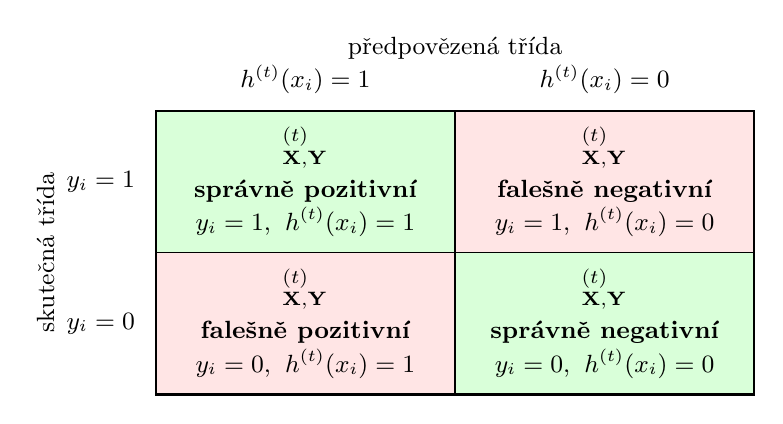
\begin{tikzpicture}[
    cell/.style={
        draw,
        minimum width=3.8cm,
        minimum height=1.8cm,
        align=center
    },
    lab/.style={font=\small},
    biglab/.style={font=\bfseries}
]

    % hlavní 2x2 tabulka
    \node[cell,biglab,fill=green!15] (tp) at (0,0)
        {$\TP_{\mathbf{X},\mathbf{Y}}^{(t)}$\\[1mm]
         \small správně pozitivní\\
         \small \(y_i=1,\ h^{(t)}(x_i)=1\)};

    \node[cell,biglab, fill=red!10] (fn) at (3.8,0)
        {$\FN_{\mathbf{X},\mathbf{Y}}^{(t)}$\\[1mm]
         \small falešně negativní\\
         \small \(y_i=1,\ h^{(t)}(x_i)=0\)};

    \node[cell,biglab, fill=red!10] (fp) at (0,-1.8)
        {$\FP_{\mathbf{X},\mathbf{Y}}^{(t)}$\\[1mm]
         \small falešně pozitivní\\
         \small \(y_i=0,\ h^{(t)}(x_i)=1\)};

    \node[cell,biglab, fill=green!15] (tn) at (3.8,-1.8)
        {$\TN_{\mathbf{X},\mathbf{Y}}^{(t)}$\\[1mm]
         \small správně negativní\\
         \small \(y_i=0,\ h^{(t)}(x_i)=0\)};

    % obrys celé tabulky
    \draw[thick] (-1.9,0.9) rectangle (5.7,-2.7);

    % popisky řádků
    \node[lab, rotate=90] at (-3.3,-0.9) {skutečná třída};
    \node[lab] at (-2.6,0) {\(y_i=1\)};
    \node[lab] at (-2.6,-1.8) {\(y_i=0\)};

    % popisky sloupců
    \node[lab] at (1.9,1.7) {předpovězená třída};
    \node[lab] at (0,1.3) {\(h^{(t)}(x_i)=1\)};
    \node[lab] at (3.8,1.3) {\(h^{(t)}(x_i)=0\)};

\end{tikzpicture}
